% -*- coding: utf-8 -*-

\chapter{Estado del arte y trabajos relacionados}
En el siguiente capítulo se realiza una presentación de los conceptos y
tecnologías que han sido utilizadas para la elaboración del proyecto y se hace
un repaso de algunos de los trabajos y aplicaciones reales que han servido de
inspiración para el diseño final del sistema.

\section{Estado del arte}
A continuación, se citan los principales elementos que constituyen la base
teórica sobre la que se sustenta el resto del escrito.

  \subsection{La tecnología \acs{RFID}}
\acs{RFID} son las siglas de \emph{Radio Frequency IDentification} (en
castellano, \emph{\textbf{identificación por radiofrecuencia}}). Se trata de un
sistema de almacenamiento y recuperación de datos remoto que utiliza las ondas
de radio para transmitir la identidad (única) de un objeto.

El modo de funcionamiento de los sistemas \acs{RFID} es simple. Una
\textbf{etiqueta \acs{RFID}} (o transponedor) que contiene datos genera una
señal de radiofrecuencia con dichos datos. Esta señal es captada por un
\textbf{lector \acs{RFID}} y este la transforma a una señal digital entendible
por una aplicación específica que utilice \acs{RFID} (figura
\ref{fig:rfidSystem}).

\begin{figure}[!h]
  \begin{center}
    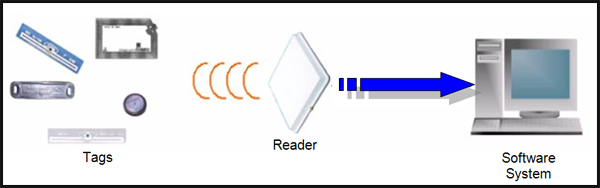
\includegraphics[width=0.8\textwidth]{rfidSystem.png}
    \caption{Esquema básico de un sistema \acs{RFID}.}
    \label{fig:rfidSystem}
  \end{center}
\end{figure}

    \subsubsection{Historia}
  El origen del \acs{RFID} está relacionado con la II Guerra Mundial. Los
  radares de la época eran capaces de detectar y medir la presencia de objetos
  dentro de un rango de actuación, pero no eran capaces de identificar qué
  clases de objetos eran identificados.

  Durante la década de los 50 y los 60, científicos de los países más
  avanzados, trabajaron para explicar cómo podrían identificar objetos
  remotamente. Fruto de estos estudios se inventaron los primeros sistemas
  antirrobo que funcionaban con ondas de radio. El objeto en cuestión tenía 
  una etiqueta con un único bit que decía si el artículo se había pagado o no.
  Cuando el objeto había sido pagado, se modificaba dicho bit, para los 
  sensores de la salida no accionaran la alarma.

  Las primeras patentes fueron solicitadas en Estados Unidos en 1973. Mario W.
  Cardullo presentó una etiqueta \acs{RFID} activa que portaba una memoria
  rescribible. Y ese mismo año, Charles Walton recibió la patente para un
  sistema \ac{RFID} pasivo, consistente en una tarjeta con un transponedor que
  comunicaba una señal a un lector situado en una puerta. Si la tarjeta era
  validada por el lector, se desbloqueaba la cerradura de la puerta.

  A partir de ese año, la tecnología \acs{RFID} empezó a utilizarse por ejemplo,
  en sistemas de apertura de puertas automáticas en centrales nucleares o en
  sistemas para controlar el ganado que había sido vacunado y el que no.

  En la década de los 90, el desarrollo de nuevos materiales permitió
  reducir drásticamente el precio de las etiquetas. Este hecho favoreció
  que se potenciara el número de aplicaciones que utilizan esta tecnología.
  Es por ello que organismos internacionales empezaran a poner sus esfuerzos en
  desarrollar estándares en el uso de este tipo de etiquetas.

    \subsubsection{Etiquetas \acs{RFID}. Arquitectura y funcionamiento}
  Las etiquetas \acs{RFID} son dispositivos pequeños, similares a una pegatina,
  que pueden incorporarse a un objeto, un animal o una persona. 
  
  Todas las etiquetas \acs{RFID} tienen en común los siguientes elementos
  (figura \ref{fig:rfidComponents}):

  \begin{figure}[!h]
    \begin{center}
      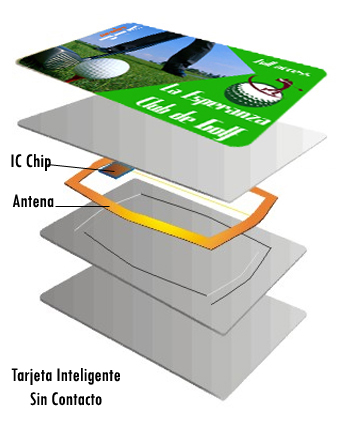
\includegraphics[width=0.4\textwidth]{rfidComponents.png}
      \caption{Componentes de una tarjeta \acs{RFID}.}
      \label{fig:rfidComponents}
    \end{center}
  \end{figure}

  \begin{itemize}
    \item \textbf{Antena}. Se encarga de recibir las señales emitidas por el
  lector y de enviar la respuesta ante dichas señales.
    \item \textbf{Chip}. Contiene la lógica de operación de la etiqueta y un
  número de identificación único.
    \item \textbf{Memoria}. Está compuesta por una parte de sólo lectura,
  que contiene las instrucciones básicas para el funcionamiento de la etiqueta;
  y por una parte de lectura y escritura, que almacena los datos escritos
  durante una comunicación con el lector.
  \end{itemize}
  
  Por otro lado, las etiquetas \ac{RFID} pueden ser de tres tipos:
  \begin{itemize}
    \item \textbf{Pasivas}. No poseen ninguna fuente autónoma de energía. La
  señal del lector es la que le induce una pequeña cantidad energía suficiente 
  como para generar y transmitir la respuesta. Tienen una fiabilidad y una
  capacidad de almacenamiento muy limitadas (unos pocos KBytes) y su campo de
  cobertura es también muy reducido (hasta 3 metros). Aún así, son las más
  utilizadas debido a su bajo coste.
   \item \textbf{Activas}. Poseen su propia fuente autónoma de energía y la
  utilizan para dar corriente a sus circuitos integrados y para propagar su
  señal al lector. Esto implica que las comunicaciones son más fiables (tienen
  menos errores), pueden transmitir señales más potentes y a mayor distancia
  (hasta 500m) y tienen más capacidad de almacenamiento. Por otro lado, tienen
  un mayor coste por chip y son de mayor tamaño que las etiquetas pasivas. La
  vida útil de sus baterías puede llegar hasta los 10 años.
    \item \textbf{Semipasivas}. Al igual que las etiquetas activas, las
  semipasivas también disponen de una fuente autónoma de energía. Sin embargo,
  estas utilizan la energía principalmente para alimentar el chip, no para
  transmitir la señal. Tienen una fiabilidad comparable a la de las etiquetas
  activas aunque superan su vida útil. Por otro lado, tienen un rango
  operativo comparable a las etiquetas pasivas aunque su respuesta es más
  rápida.
  \end{itemize}

    \subsubsection{Lectores RFID. Funcionamiento}
  Los lectores \acs{RFID} son los encargados de leer o re-escribir la
  información almacenada en las etiquetas.
  El funcionamiento es sencillo. La antena del lector crea un campo magnético
  y cuando este campo entra en contacto con una etiqueta, se produce la
  reacción de esta última, enviando al lector la información contenida.
  El lector decocifica los datos obtenidos y los manda a una tercera entidad 
  para que los interprete (figura \ref{fig:rfidSchema}).

  \begin{figure}[!h]
    \begin{center}
      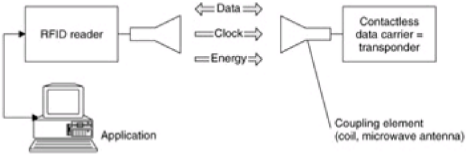
\includegraphics[width=0.8\textwidth]{rfidSchema.png}
      \caption{El lector y la etiqueta son los principales componentes de todo
sistema \acs{RFID}.}
      \label{fig:rfidSchema}
    \end{center}
  \end{figure}

  Según el número de bobinas que poseen, existen dos tipos de lectores:
  \begin{itemize}
  \item \textbf{Bobina simple}. La misma bobina crea el campo magnético y
  transmite los datos. Son las más simples y baratas que las dobles y tienen
  un alcance muy limitado.
  \item \textbf{Bobina doble}. Una de las bobinas se encarga de crear el
  campo magnético y la otra de transmitir los datos. Son caras pero tienen
  mayores prestaciones que las bobinas simples.
  \end{itemize}
  
  En cuanto a la portabilidad, también existen dos tipos de lectores:
  \begin{itemize}
  \item \textbf{Lectores móviles}. Son lectores autónomos que pueden 
  transportarse a cualquier lugar y que pueden utilizarse con varios fines. Se
  comunican con otros dispositivos a través de conexiones inalámbricas.
  \item \textbf{Lectores fijos}. Son lectores ubicados en un punto fijo y 
  dedicados a un único fin. Tienen mayor rango de actuación que los lectores
  móviles y suelen utilizarse en sistemas de detección y seguimiento de
  personas y animales.
  \end{itemize}

    \subsubsection{La tecnología \emph{MIFARE}}
  \emph{MIFARE} es el estándar de la industria para interfaces de
  tarjetas inteligentes sin contacto y lectores que operan a 13.56MHz.
  Funcionan de acuerdo con el estándar \acs{ISO} 14443\cite{bib:mifare}.
  
  El alcance típico de lectura/escritura de etiquetas \emph{MIFARE} sin
  contacto oscila entre los 2 y los 10 cm; y la capacidad más habitual está
  entre los 1 y los 4KB de memoria \acs{EEPROM}.

  Para que los datos sean leídos o escritos es necesaria una autentificación 
  mútua entre el lector y la etiqueta, ya que el acceso a los mismos está 
  protegidos por una clave de 48 bits. La transmisión de datos por
  radiofrecuencia viaja encriptada.

  En la actualidad \emph{MIFARE} es una marca registrada de \emph{NXP
  Semiconductors} (empresa fundada por \emph{Philips}). Ha vendido más de 5 mil
  millones de tarjetas y etiquetas inteligentes y más de 50 millones de
  componentes de lectores. Ha sido seleccionada seleccionada para la mayoría
  de proyectos importantes con tarjetas inteligentes sin contacto en todo el
  mundo y su cartera de productos incluye soluciones perfectas para la
  recaudación automática de tarifas, tarjetas de fidelización, cobro en 
  carreteras de peaje o gestión de acceso a edificios\cite{bib:urlMifare} 
  (figura \ref{fig:mifareFamily}.

  \begin{figure}[!h]
    \begin{center}
      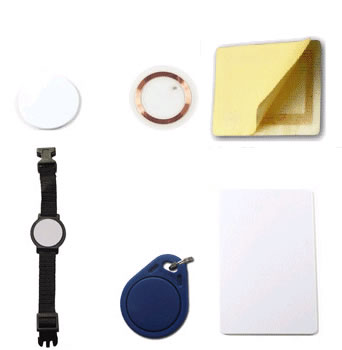
\includegraphics[width=0.5\textwidth]{mifareFamily.png}
      \caption{Ejemplos de etiquetas MIFARE.}
      \label{fig:mifareFamily}
    \end{center}
  \end{figure}

  \subsection{La tecnología NFC}
  \subsection{La tecnología Bluetooth}
  \subsection{Los servicios web}
  \subsection{El framework .NET}
  \subsection{La tecnología Java}
  \subsection{Los displays táctiles}
  \subsection{La computación móvil}

\section{Trabajos relacionados}
  \subsection{Estudios relacionados}
    \subsubsection{Modelos de comercio utilizando NFC}
    \subsubsection{Métodos de pago móvil}
    \subsubsection{Métodos de fidelización de clientes}

  \subsection{Aplicaciones comerciales}
    \subsubsection{Gestión de operaciones típicas de un restaurante}
    En la actualidad existe una innumerable oferta de aplicaciones que ayudan
    a gestionar las labores típicas de un restaurante: gestionar pedidos,
    generar facturas, realizar la función de caja registradora, \dots
      \begin{itemize}
      \item \emph{\textbf{\href{http://www.softrestaurant.com/}
      {SoftRestaurant}}}. Es un software desarrollado por la empresa mexicana ç
      \emph{\href{http://www.nationalsoft.com.mx/}{National Soft}}.
      Actualmente va por la versión \emph{8.0}.

      % Descripción general y foto

      A diferencia de otros programas de gestión de restaurantes, permite
      describir las recetas de los productos contemplados en la carta. Es 
      decir, permite listar los ingredientes (con sus cantidades) utilizados
      en la elaboración de cada plato, pudiendo además gestionar el
      \emph{stock} de esos ingredientes.

      \item \emph{\textbf{\href{http://www.estudiolegaspi.com.ar/Salewin.html}
      {SaleYa}}}. Es un software desarrollado por la empresa argentina 
      \emph{\href{http://www.estudiolegaspi.com.ar/}{Estudio Legaspi}}.
      Dispone de una versión limitada de prueba.

        % Descripción general y foto

      Permite editar los objetos (mesas, barra, \dots) que conforman la vista 
      del restaurante, para simular la planta del restaurante real. Además, las
      mesas son representadas con un color u otro según su estado (libre u
      ocupada).

      \item \emph{\textbf{\href{http://www.restbar.com/}{RestBar}}}. Es un
      software desarrollado por la empresa mexicana
      \emph{\href{http://www.ambit.com.mx/}{Ambit Tecnology}}. Actualmente se
      encuentra en la versión \emph{12.03a}.

      % Descripción general y foto

      Dispone de un monitor de comandas (situado en la cocine) que permite
      gestionar el estado de elaboración de los platos.

      \item \emph{\textbf{
      \href{http://www.icg.es/?es/software-programas/restaurantes-hosteleria}
      {FrontRest}}}. Es un software desarrollado por la empresa española
      \emph{\href{http://www.icg.es}{ICG Software}}.

      Dispone de varios módulos que satisfacen las necesidades de información
      del restaurante: aplicaciones móvil para repartos a domicilio, aplicación
      para gestionar los pedidos en la barra, aplicación móvil para tomar nota
      de los pedidos de las mesas, impresora de comandas (para comunicación 
      con la cocina), gestión del \emph{stock} de productos en el almacén, 
      \dots
      \end{itemize} 
    \subsubsection{Gestión de pedidos a través de dispositivos móviles}
      \begin{itemize}
      \item \textbf{vMenu}
          % Los clientes pueden realizar pedidos desde su mesa a través de un
          %dispositivo móvil o fijo.
      \item \textbf{Brand Table}
          % la mesa de restaurante NFC que quiere eliminar al cajero de la
          %ecuación.
      \end{itemize}
    \subsubsection{Gestión de pagos}

% Local Variables:
%   coding: utf-8
%   mode: latex
%   mode: flyspell
%   ispell-local-dictionary: "castellano8"
% End:
